% This is my HW 6 solution set.

\documentclass[12pt, leqno]{article}
\usepackage{amsfonts, amsmath, amssymb}
\usepackage{fancyhdr}
\usepackage{hyperref}
\usepackage{graphicx}
\newcounter{qcounter}
\usepackage[lofdepth,lotdepth]{subfig}
\usepackage[maxfloats=40]{morefloats}
\usepackage{float}
\usepackage{}
\usepackage[english]{babel}
\usepackage{tabularx}
\providecommand{\abs}[1]{\lvert#1\rvert} % absolute value
\providecommand{\normd}{\mathcal{N}} % normal distribution
\providecommand{\norm}[1]{\lVert#1\rVert} % norm
\newcommand{\macheps}{\epsilon_{\mbox{\scriptsize mach}}}
\usepackage[ampersand]{easylist}
\makeatletter
\newcommand{\distas}[1]{\mathbin{\overset{#1}{\kern\z@\sim}}}%
\newsavebox{\mybox}\newsavebox{\mysim}
\newcommand{\distras}[1]{%
  \savebox{\mybox}{\hbox{\kern3pt$\scriptstyle#1$\kern3pt}}%
  \savebox{\mysim}{\hbox{$\sim$}}%
  \mathbin{\overset{#1}{\kern\z@\resizebox{\wd\mybox}{\ht\mysim}{$\sim$}}}%
}
\makeatother

\begin{document}
\pagestyle{fancy}
\lhead{Syed Rahman}
\rhead{STA6866}

\begin{center}
{\large {\bf Homework 7}} \\
\end{center}
\paragraph{1.} 

\begin{table}[ht]
\centering
\scalebox{0.8}{
\begin{tabular}{rlrrrr}
  \hline
 & Player & True Value & Stein & Efron-Morris& Posterior Means \\ 
  \hline
1 & Clemente,Roberto & 0.35 & 0.29 &0.334& 0.31 \\ 
  2 & Robinson,Frank & 0.30 & 0.29 &0.313& 0.30 \\ 
  3 & Howard,Frank & 0.28 & 0.28 &0.292& 0.29 \\ 
  4 & Johnstone,Jay & 0.22 & 0.28 &0.277& 0.29 \\ 
  5 & Berry,Ken & 0.27 & 0.27 &0.334&0.273 0.28 \\ 
  6 & Spencer,Jim & 0.27 & 0.27 &0.273& 0.28 \\ 
  7 & Kessinger,Don & 0.26 & 0.27 &0.268& 0.27 \\ 
  8 & Alvarado,Luis & 0.21 & 0.26 &0.264& 0.27 \\ 
  9 & Santo,Ron & 0.27 & 0.26 &0.259& 0.26 \\ 
  10 & Swaboda,Ron & 0.23 & 0.26 &0.259& 0.26 \\ 
  11 & Petrocelli,Rico & 0.26 & 0.25 &0.254& 0.25 \\ 
  12 & Rodriguez,Ellie & 0.23 & 0.25 &0.254& 0.25 \\ 
  13 & Scott,George & 0.30 & 0.25 &0.254& 0.25 \\ 
  14 & Unser,Del & 0.26 & 0.25 &0.254& 0.25 \\ 
  15 & Williams,Billy & 0.33 & 0.25 &0.254& 0.25 \\ 
  16 & Campaneris,Bert & 0.28 & 0.25 &0.249& 0.24 \\ 
  17 & Munson,Thurman & 0.32 & 0.24 &0.244& 0.24 \\ 
  18 & Alvis,Max & 0.20 & 0.24 &0.239& 0.23 \\ 
   \hline
\end{tabular}
}
\end{table}


\begin{figure}
\begin{center}
  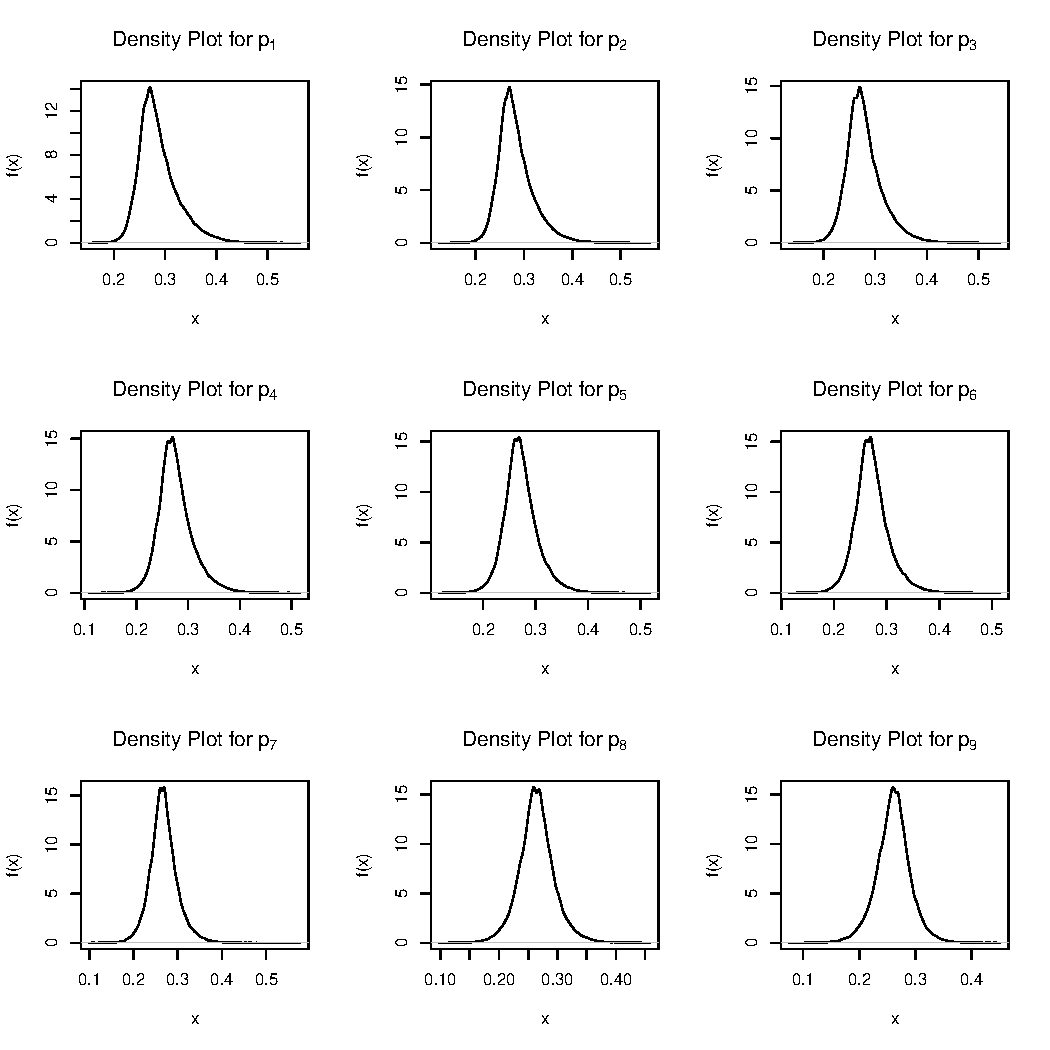
\includegraphics[scale=0.65]{pdensity1.pdf}
\end{center}
\caption{Posterior Density plots for $p_i, i = 1, ..., 9$} 
\label{density1}
\end{figure} 

\begin{figure}
\begin{center}
  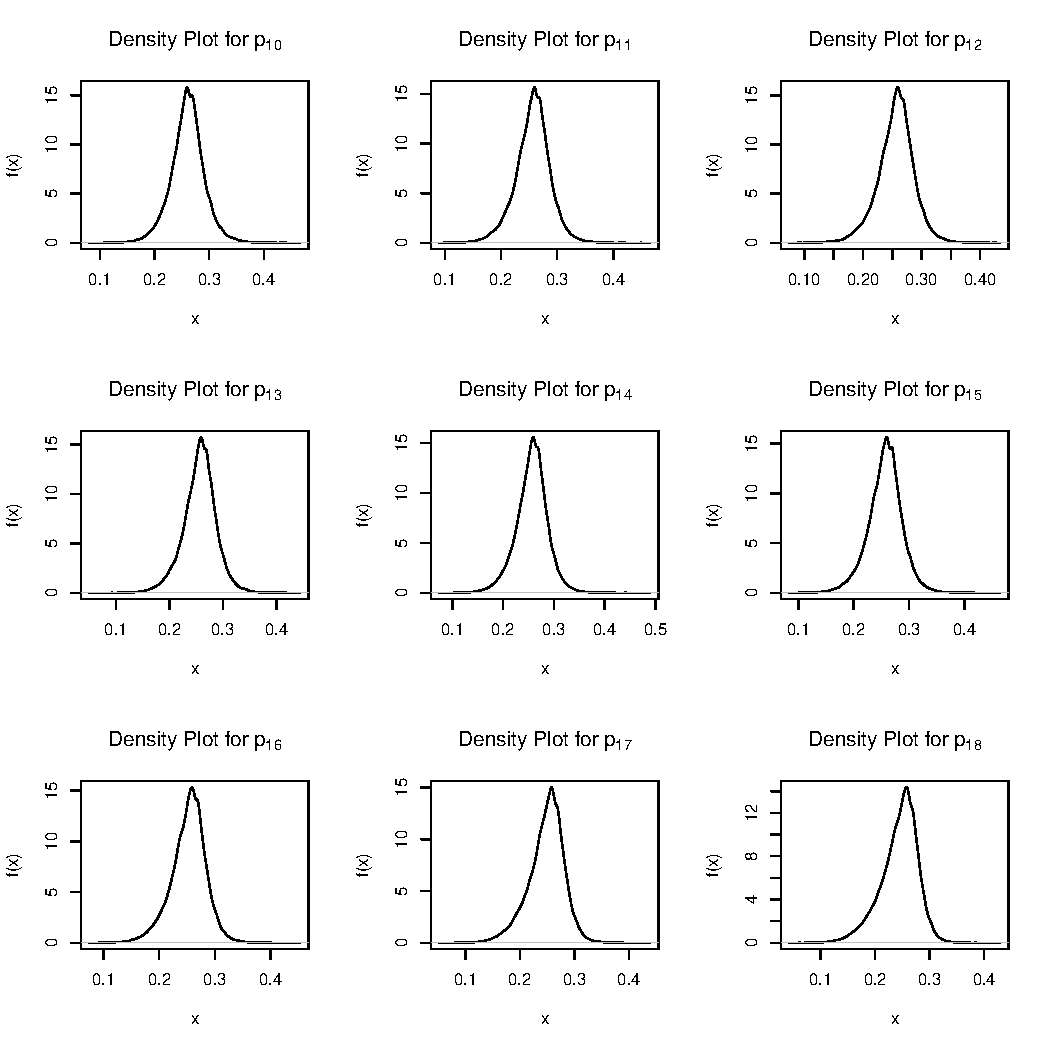
\includegraphics[scale=0.65]{pdensity2.pdf}
\end{center}
\caption{Posterior Density plots for $p_i, i = 1, ..., 9$} 
\label{density2}
\end{figure} 

 
\pagebreak

\paragraph{Appendix 1: model.txt}
\begin{verbatim}

\end{verbatim}

\paragraph{Appendix 2: script.txt}
\begin{verbatim}

\end{verbatim}

\paragraph{Appendix 3: R code}

\begin{verbatim}

\end{verbatim}
\end{document}